%-------------------------------------------------------------------------
\subsection{McWhorter problem}

It is assumed that the flow of both wetting and non-wetting phases can be adequately described by Darcy's law if the phases are immiscible and incompressible

\begin{equation}
n\frac{\partial S^{\gamma}}{\partial t} + \nabla \cdot \mathbf{q}^{\gamma} = 0, \gamma=w, nw
\label{eq:mcwtMassEq}
\end{equation}
\begin{equation}
\mathbf{q}^{\gamma}=-{\mathbf K} \lambda^{\gamma} \nabla p^{\gamma}
\label{eq:mcwtFluxEq}
\end{equation}

where $\lambda_w$ and  $\lambda_{nw}$ are mobility of the wetting and non-wetting fluid. Both phase are linked by the state equation $S_w+S_{nw}=1$ and $p_c=p_g-p_w$. Here total flux, $\mathbf {q}_t=\mathbf {q}_w + \mathbf {q}_{nw}$ and $p_c$ is a function of $S_w$.

A formulation that is often used for two phase flow problems is the so-called fractional flow model. The attractiveness of this formulation is that the model becomes more accessible to analysis. Subtracting equation ($18.1.24$) for both phases we have

\begin{equation}
\mathbf {q}_w=f \mathbf {q}_t- D \frac{\partial S_w}{\partial x}
\label{eq:McWhorterWetFlux}
\end{equation}

where 

\begin{equation}
f=\frac{1}{1 + \frac{\lambda_{nw}}{\lambda_w}},~~~D=-\lambda_{nw} f \frac{\partial p_c}{\partial S_w}.
\end{equation}

The first term on the right of equation (\ref{eq:McWhorterWetFlux}) dictates the rate at which flux is injected on the boundary and the second term represent the additional force due to the gradient of capillary pressure. Inserting equation (\ref{eq:McWhorterWetFlux}) into equation (\ref{eq:mcwtMassEq}) for the wetting phase and assuming that total flux, $\mathbf q_t$ is space invariant

\begin{equation}
\frac{\partial }{\partial x}\left( D\frac{\partial S_w}{\partial x}\right) - \mathbf q_t \frac{\partial f}{\partial S_w}\frac{\partial S_w}{\partial x}=n \frac{\partial S_w}{\partial t}.
\label{eq:McWhorterAnal}
\end{equation}

In the last benchmark (Buckley and Leveret) it is assumed that teh force due to the gradient of capillary pressure is very small relative to total flux, $\mathbf q_t$, and hence the second order term is suppressed in the equation.

Including capillarity, model verification can occur against the analytical solution of McWhorter and Sunada ($1990$). They developed an exact quasi-analytical solution of equation (\ref{eq:McWhorterAnal}) for unidirectional displacement of a non-wetting phase by a wetting phase using the concept of a fractional flow function.

The fractional flow function is defined as the ratio of wetting phase flux, $\mathbf q_w$ to the total flux, $\mathbf q_t$. It has been shown that this ratio is function of $S_w$ only, when $\mathbf q_t$ is inversely related to square root of the time.

\subsubsection*{Definition}
The test benchmark problem for capillary effects is formulated as if the instantaneous displacement occurs in a one-dimensional horizontal reservoir initially occupied by oil. Solution has been obtained by solving the governing equations (\ref{eq:msbl_sim}) by the pressure-pressure scheme described above. Different from the Buckley-Leverett problem, here flow is governed by capillary forces when water saturation at the left end of the horizontal column is kept to be one, while the right end is kept to be zero flux. Therefore, no source term exists, and flow is by capillary force alone.

\begin{figure}[!tbh]
\begin{center}
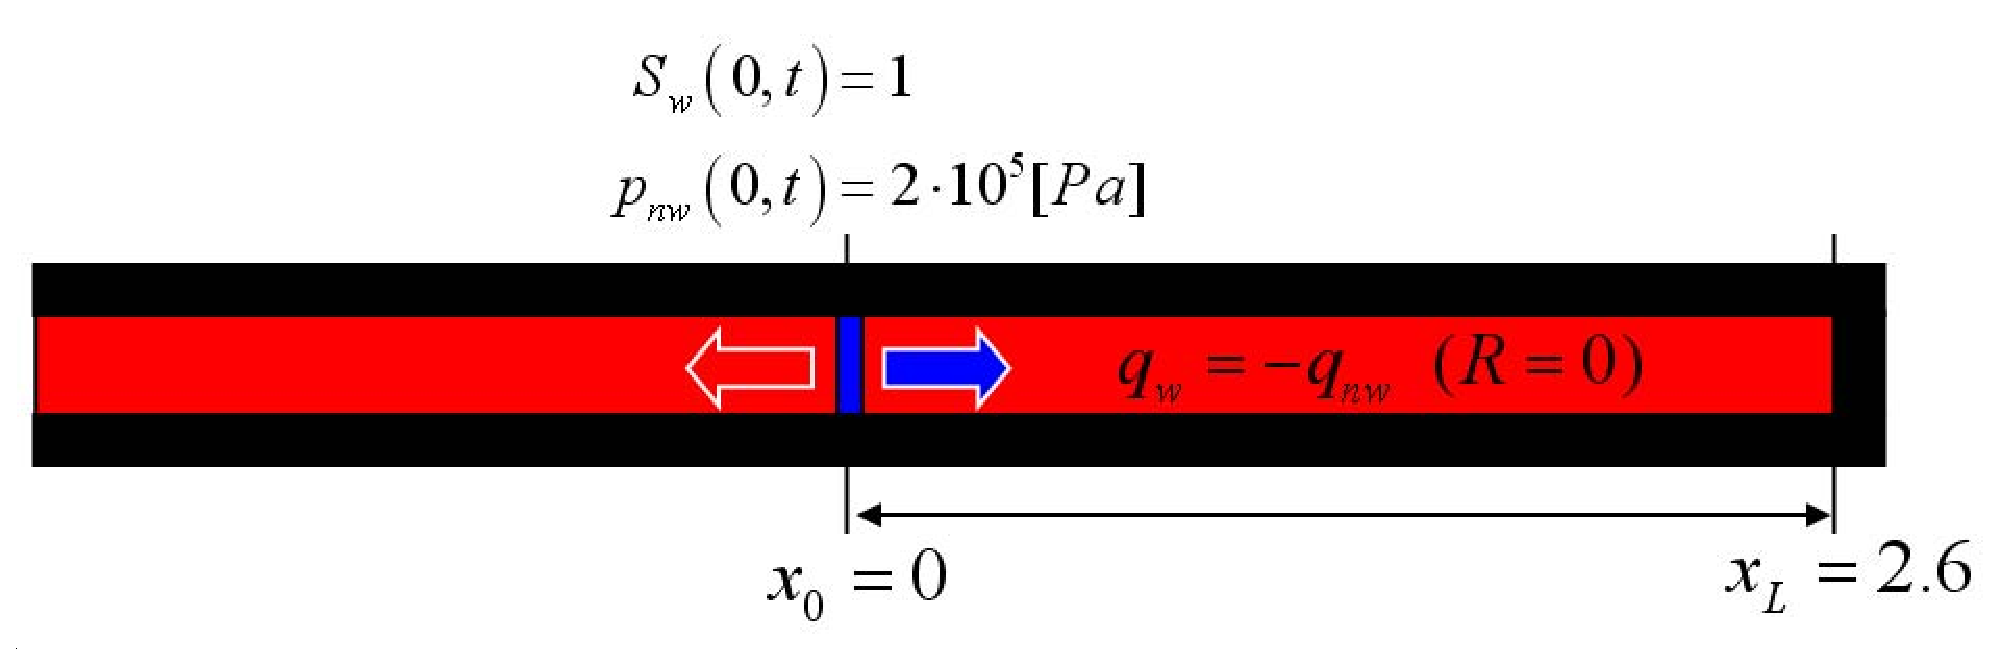
\includegraphics[height=3cm]{chapter_13/figures/fig_13_1_9}
\end{center}
\caption{Schematic of the benchmark formulated to test McWhorter and Sunada's analytical solution.}
\label{mcwt:config}
\end{figure}

\subsubsection*{Results}
Based on the above discussion OpenGeoSys produces an agreeable solution. Fig. \ref{mcwt:ppModel} shows the water saturation profile, $S_w$ with a fine grid along with $2.6m$ long horizontal column for different time steps. Line elements have been used with the time and space discretization $\delta t=0.5s$ and $\delta x=0.05m$ respectively.

\begin{figure}[!tbh]
\begin{center}
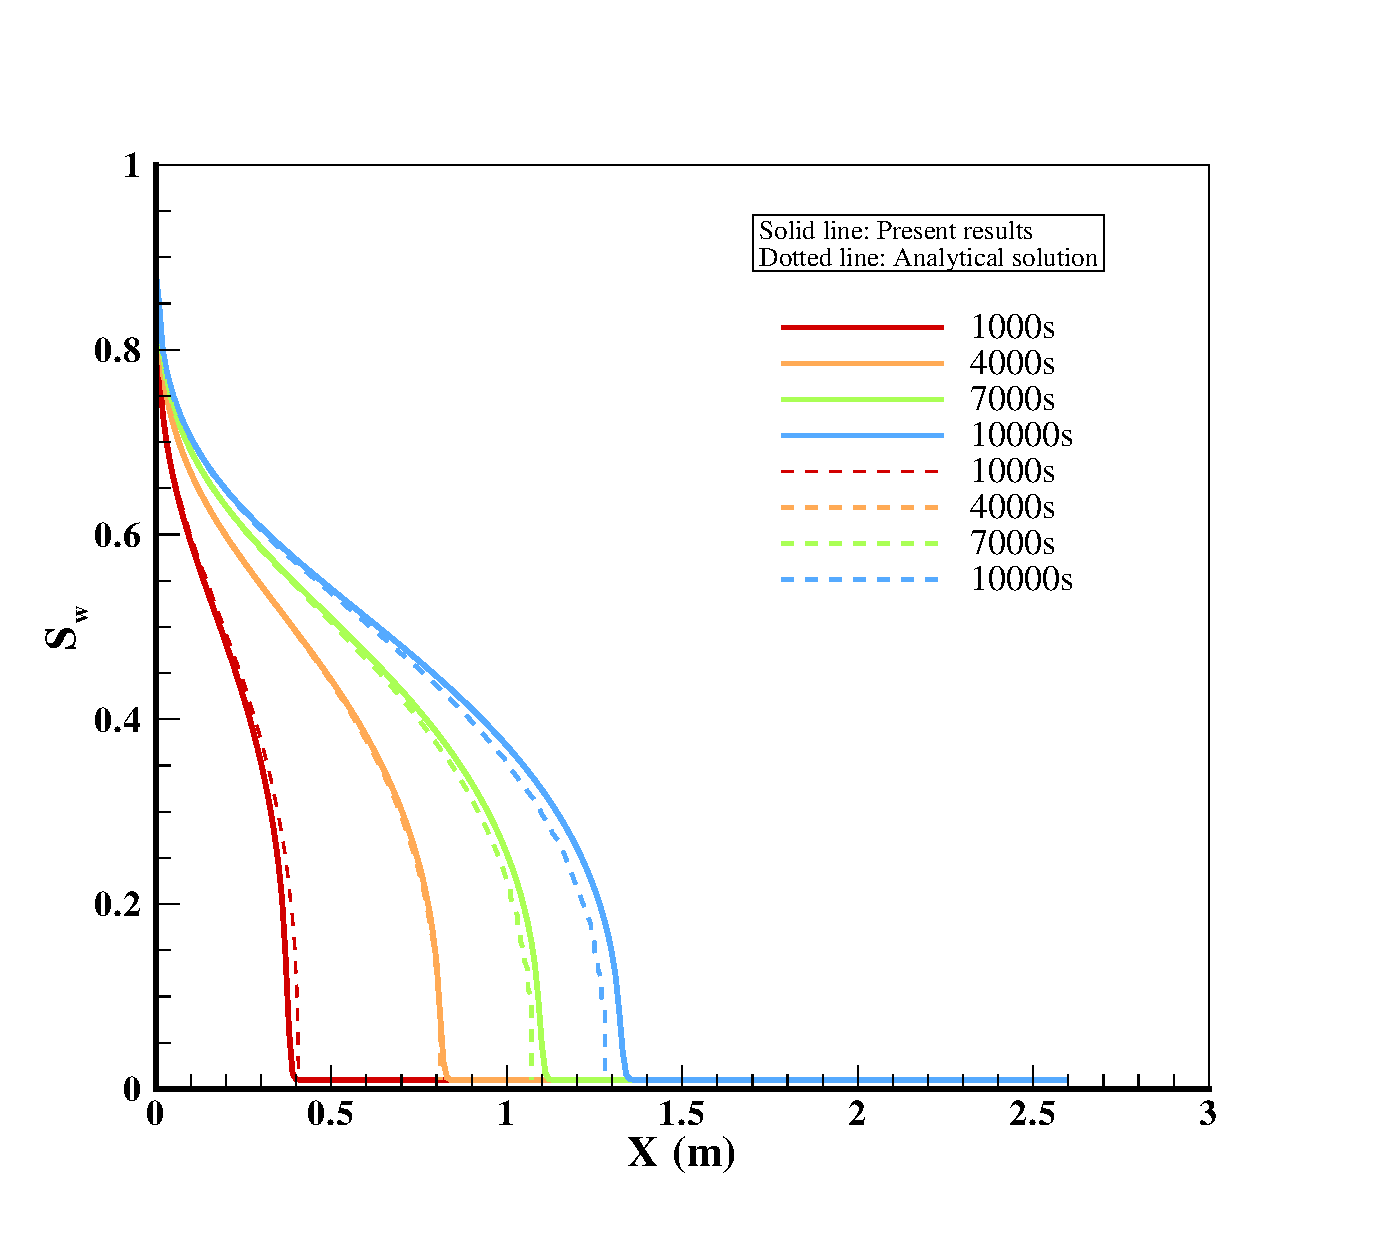
\includegraphics[width=0.7\textwidth]{chapter_13/figures/fig_13_1_10}
\end{center}
\caption{Water saturation, $S_w$ profile of the present result along with analytical solution based on one by McWhorter.}
\label{mcwt:ppModel}
%\end{figure}
%\begin{figure}[!htb]
\begin{center}
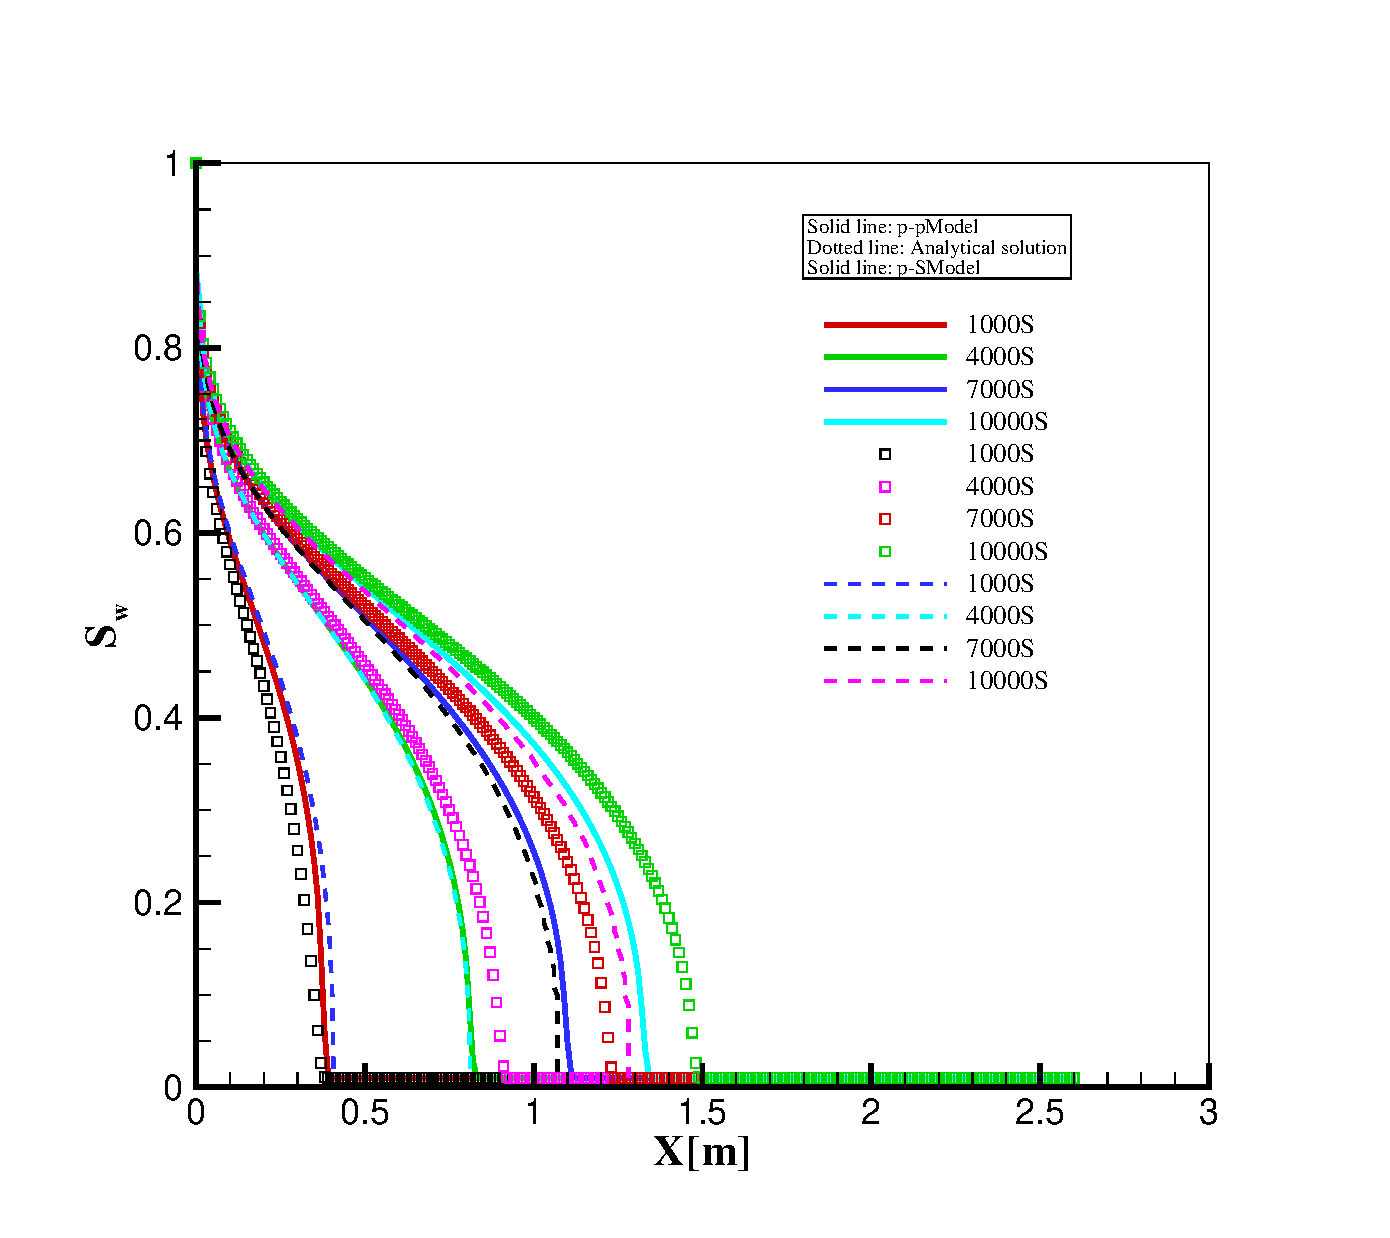
\includegraphics[width=0.7\textwidth]{chapter_13/figures/fig_13_1_11}
\end{center}
\caption{Water saturation, $S_w$ profile in sequential iterative coupling scheme.}
\label{mcwt:psModel}
\end{figure}

Next, we solve exactly same problem using the total pressure based pressure-saturation model in a sequential iterative coupling scheme. Unlike the pressure-pressure model, one downside for the total-pressure-based saturation model is that it is less accurate for problems dominated by capillarity (see Fig. \ref{mcwt:psModel}). Since the pressure-pressure model directly solves for capillary pressure as a primary variable, the model has an advantage for the capillary related problems. On the other hand, the total-pressure-based saturation model is limited to the problems when $d P_c/d S_w$ is close to zero. The condition for $d P_c/d S_w$ close to zero is caused physically in the case of fractures, shear zones, and transitions between heterogeneities.

\begin{table}[!htb]
\begin{tabular}{lccr}
\hline\noalign{\smallskip}
Property & Symbol & Value & Unit \\
\noalign{\smallskip}\hline\noalign{\smallskip}
Column length & $L$ & $m$ & $2.6$  \\
wetting dynamic viscosity &  $\mu_w$ & $Pa.s$ & $1.0\times10^{-3}$ \\
non-wetting dynamic viscosity & $\mu_{nw}$ & $Pa.s$ & $1.0\times10^{-3}$ \\
wetting phase density &  $\rho_w$ &$kg.m^{-3}$ & $1.0\times10^{3}$ \\
Non-wetting phase density &  $\rho_{nw}$ & $kg.m^{-3}$ & $1.0\times10^{3}$ \\
Permeability & $\mathbf K$ & $ m^2$ & $1.0\times 10^{-10}$ \\
Porosity & $n$ & $--$ & $3.0\times10^{-1}$ \\
Residual saturation of water &  $S_{rw}$ & $--$ & $0$ \\
Residual saturation of oil &  $S_{nrw}$ & $--$ & $0$ \\
Entry pressure &  $p_d$ & $Pa$ & $5.0\times10^{3}$ \\
Soil distribution index &  $\lambda$ & $--$ & $2.0$ \\
Capillary pressure & $p^c(S_{eff})$ & $Pa$ & Brooks-Corey model\\
Relative permeability & $\kappa_{rel}(S_{eff})$ & $--$ & Brooks-Corey model \\
\noalign{\smallskip}\hline
\end{tabular}
\caption{Material parameters for the McWhorter problem.}
\end{table}
